\begin{figure}[htbp]
    \centering
    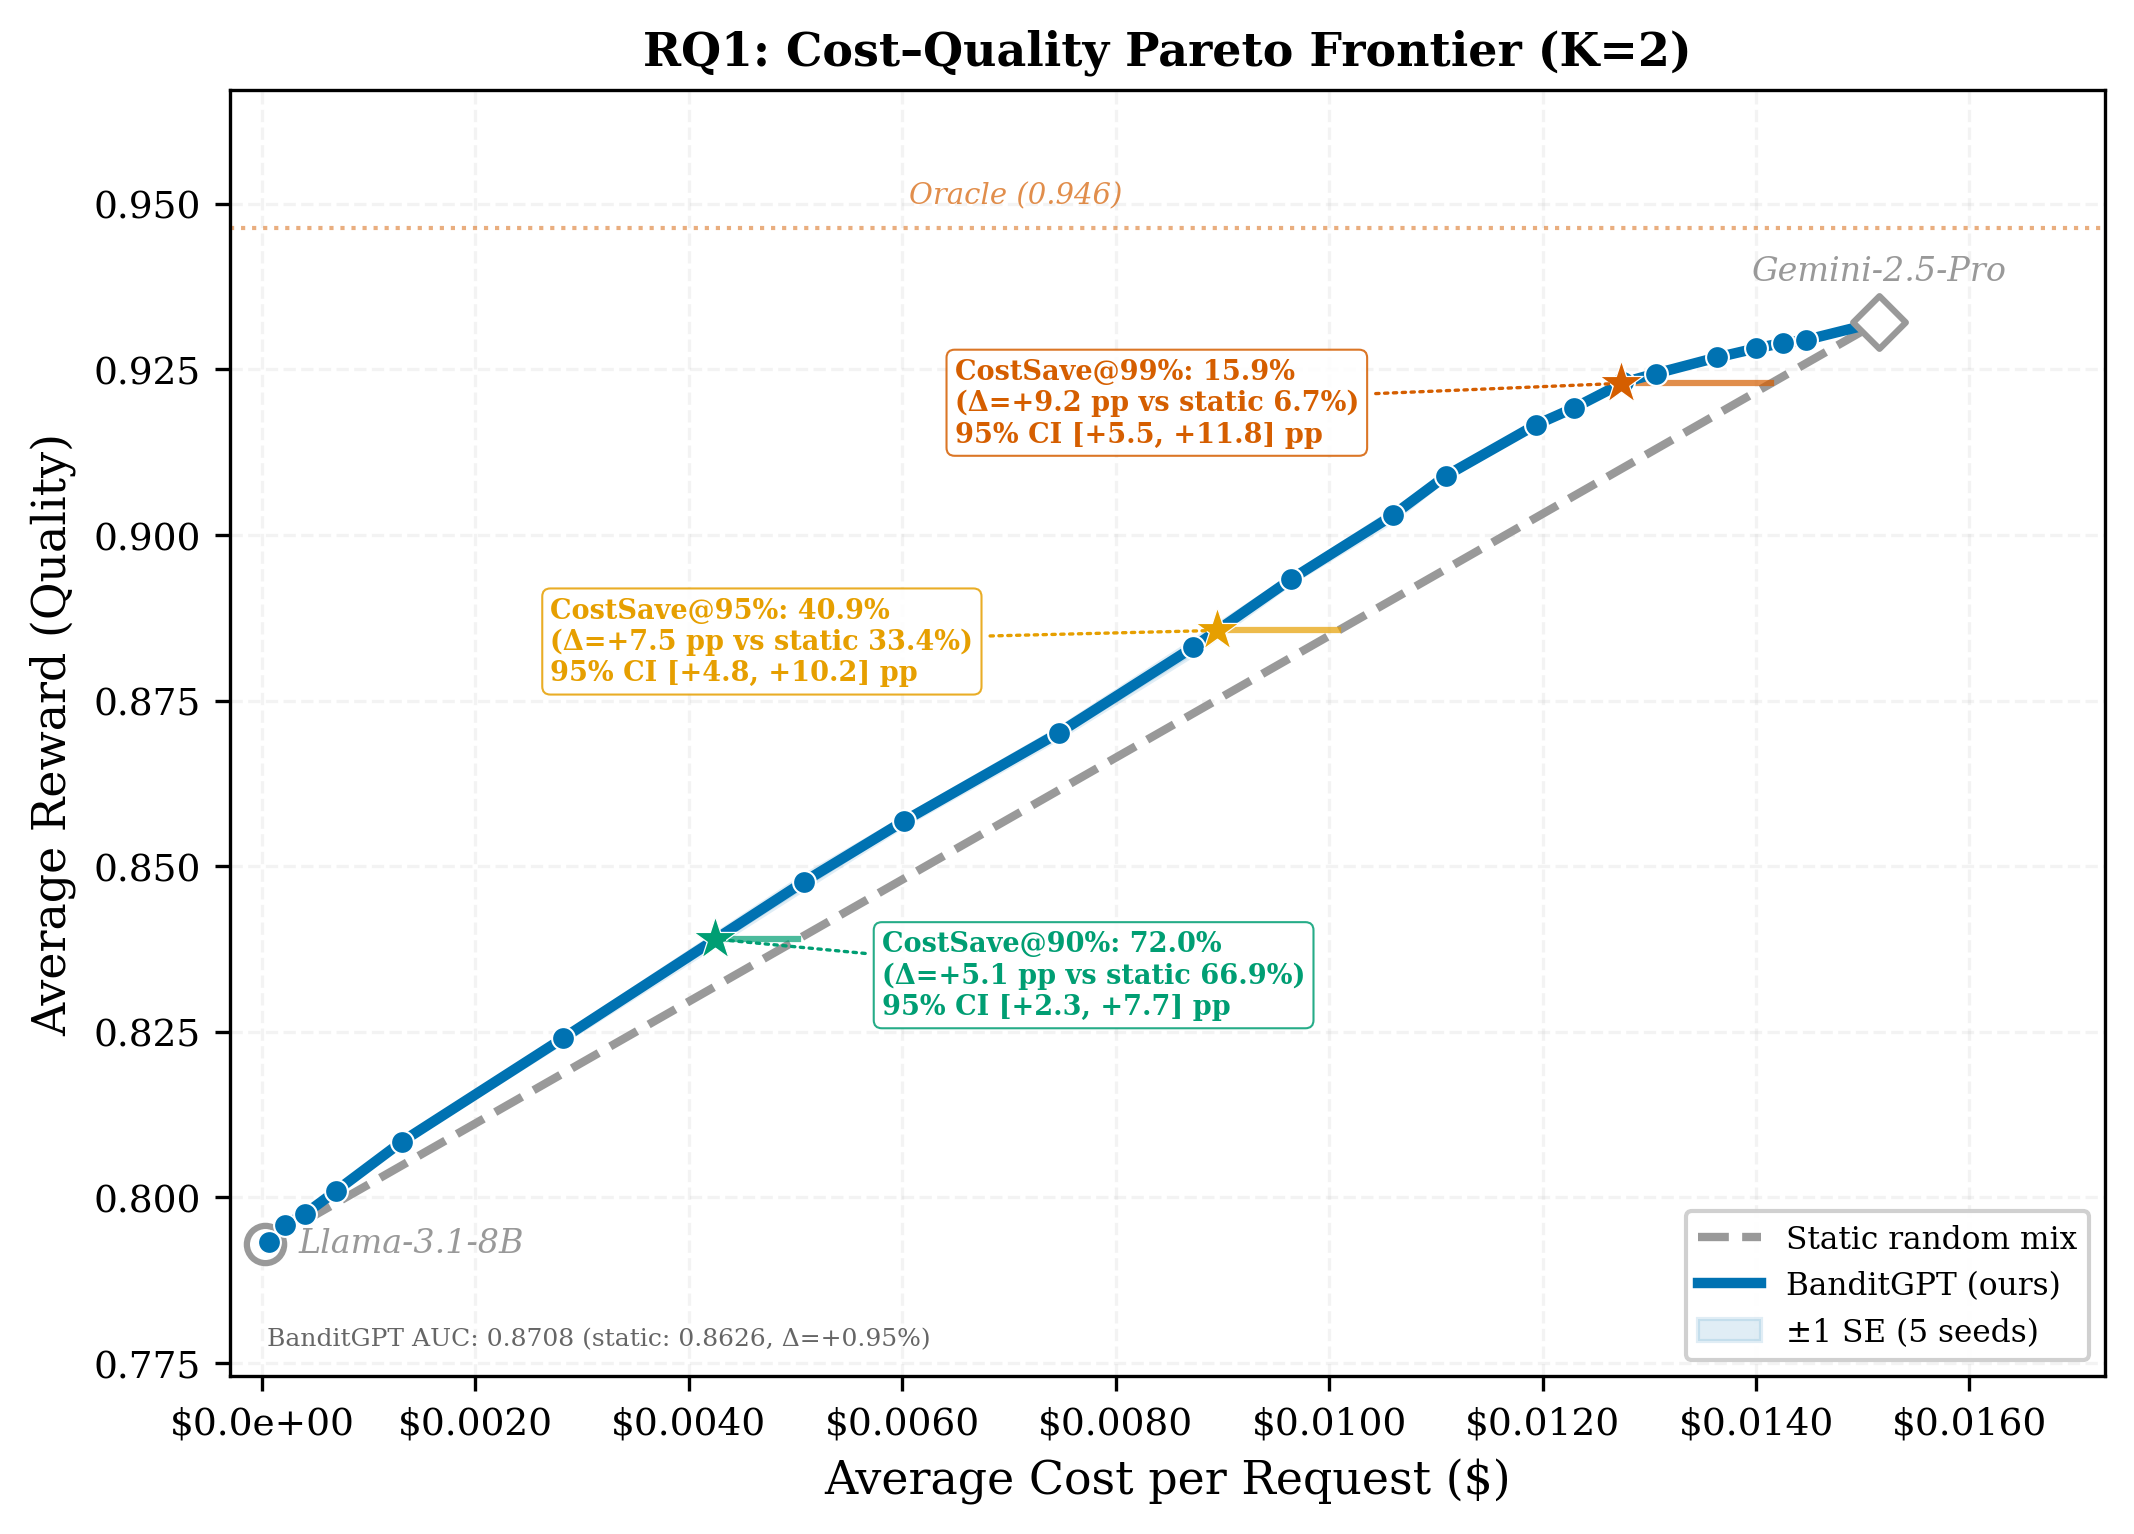
\includegraphics[width=\linewidth]{../experiments/01_figure/results/figure1_pareto_k2.pdf}
    \caption{Cost--quality Pareto frontier for the $K{=}2$ portfolio
    (\texttt{Llama-3.1-8B} at \$0.00003/req vs.\
    \texttt{Gemini-2.5-Pro} at \$0.015/req; $500{\times}$ cost ratio).
    %
    \textbf{Solid blue curve:}\ \textit{banditGPT} frontier traced by
    sweeping cost penalty $\lambda$ over 22 values in $[0,\,10]$,
    averaged over 5~seeds; shaded band shows $\pm 1$~SE\@.
    The bandit receives only \emph{partial feedback} (the reward for
    the model it chose) and continues learning during the test phase.
    %
    \textbf{Dashed red:}\ supervised logistic regression
    (val-tuned $C{=}0.1$), trained with \emph{full reward labels} for
    all models on every prompt---strictly more information than any
    bandit.  Despite this advantage, \textit{banditGPT}
    matches its frontier (AUC $0.870$ vs.\ $0.869$).
    %
    \textbf{Other bandit variants} ($\varepsilon$-greedy, LinTS,
    tabula~rasa LinUCB; all val-tuned) cluster within
    ${\approx}\,0.1\%$ AUC of \textit{banditGPT}, confirming that
    for a two-arm portfolio the routing problem is learnable by any
    contextual method.
    %
    \textbf{Context-free UCB} (dotted green) collapses to the
    \textbf{static random-mix} baseline (dashed gray), demonstrating
    that without prompt-level features a bandit can only choose a
    global mixing ratio---no better than flipping a biased coin.
    %
    \textbf{Star markers:}\ CostSave\,@\,$Q$ at quality thresholds
    $Q \in \{90\%,\, 95\%,\, 99\%\}$
    (Table~\ref{tab:costsave_k2}).
    At the 95\% quality threshold the bandit saves
    41.5\% of cost vs.\ 33.4\% for static mixing
    ($\Delta{=}+8.1$~pp, $95\%$~CI: $[+5.1,\;+10.8]$).
    %
    Setup: train $n{=}8{,}374$, val $n{=}1{,}785$, test
    $n{=}1{,}824$ prompts;
    rewards from DeepSeek-R1~\cite{deepseekai2025deepseekr1}
    (see Section~\ref{sec:reward_assumption}).
    All baseline hyperparameters selected on val by Pareto AUC.
    }
    \label{fig:pareto_k2}
\end{figure}
